\documentclass[12pt]{article}

\usepackage{fancyhdr}
\usepackage{geometry}
\usepackage{ucs}
\usepackage[utf8x]{inputenc}
\usepackage[T1]{fontenc}
\usepackage[english]{babel}
\usepackage{amsmath,amssymb,amstext}
\usepackage{hyperref}
\usepackage{cancel}
\usepackage{dsfont}
\usepackage{physics}
\usepackage{lmodern}
\usepackage{enumerate}
\usepackage{enumitem}
\usepackage{graphicx}
\usepackage{listings, color}
\usepackage[labelfont=bf]{caption}
\usepackage{titling}


\lstset{basicstyle=\scriptsize,breaklines=true} %Quellcode mit Umlauten und ganz klein

\lstset{literate=
  {Ö}{{\"O}}1
  {Ä}{{\"A}}1
  {Ü}{{\"U}}1
  {ß}{{\ss}}2
  {ü}{{\"u}}1
  {ä}{{\"a}}1
  {ö}{{\"o}}1
}


%Geometrie----------------------------------------------------------------------------------------------------------

\geometry{a4paper, top=25mm, left=15mm, right=15mm, bottom=25mm,headsep=10mm, footskip=10mm}
\pagestyle{fancy}
\setlength{\parindent}{0pt} %Zeileneinrückung

\fancyhf{} %Setzt voreingestellte Kopf-und Fußzeilen-Eigenschaften zurück

\lhead{\nouppercase{\leftmark}}
\chead{}
\rhead{\thepage}

\lfoot{}
\cfoot{}
\rfoot{}

\title{\vspace{0cm}{\Huge Fortgeschrittenen-Praktikum I:\\ \vspace{1cm} LHWZ}}
\author{Saskia Bondza\\Simon Stephan}
\date{Durchgeführt am 02.09.2016 und 05.09.2016}

\pretitle{%
  \begin{center}
  \LARGE
  
\includegraphics[width=6cm,]{figures/siegel}\\[\bigskipamount]
}
\posttitle{\end{center}}

%neue Commands----------------------------------------------------------------------------------------------------------
\newcommand{\nab}{\vec{\nabla}} %direkter Befehl mit Vektorpfeil
\newcommand{\gra}[3][0.7]{
	\begin{minipage}[h!]{\textwidth}
		\centering
		\includegraphics[width=#1\textwidth]{figures/#2.png}
		\captionof{figure}{#3}
	\end{minipage}
	\vskip 30 pt
	}

\newcommand{\del}[2][]{\frac{\partial #1}{\partial #2}}
\newcommand{\code}[1]{\texttt{#1}}

%Titel,Inhalt----------------------------------------------------------------------------------------------------------

\begin{document}
\pagenumbering{gobble} %verstecke Seitenzahl
\maketitle
\newpage

\section*{Abstract}

\newpage

\thispagestyle{empty}
\tableofcontents
\newpage

%Schreiben----------------------------------------------------------------------------------------------------------
\pagenumbering{arabic} %verstecke Seitenzahl
\section{Introduction}
In order to determine the half life of a radioactive elements, usually the number of decays per second (decay rate) is measured and the change over time of the decay rate observed. The half-life can then be determined from this characteristic exponential behaviour. However, this method isn't useful to determine the half-life of samples with a very long half-life, e.g. ${}^{238}$Uranium with a half-life of $T_{1/2}$=4,468$\cdot 10^9$years,  as hardly any change will be observed. Instead the activity of the sample is measured, that presents the quantity describing the derivative of the law of decay given by the following relation: A=$\dot{N}$=ln2N/$T_{1/2}$ where N is the known number of radioactive nuclides.


In this experiment this method is used to determine the half-life of the $\alpha$-emitter ${}^{147}$Samarium and the $\beta$-emitter ${}^{40}$Kalium both having very long half-lives. Additionally two different correction procedures are applied to consider back-scattering and self-absorption effects. 
In the case of Samarium, we take advantage of the constant range of the  $\alpha$-radiation and the known surface area while we make use of the mass dependency for Kalium.
%Bei Samarium wird die konstante Reichweite der $\alpha$-Strahlung und die bekannte Oberflächengröße ausgenutzt und bei Kalium die Massenabhängigkeit.











\newpage
\section{Theoretical Background}

\subsection{Law of decay}\label{zerfallsgesetz}

Radioactive Decay is a stochastic process which implies that the exact point of time at which a single atom decays can not be predicted, but only a probability that it will decay for any given point in time.  
The decay rate $frac{dN}{dt}$ for a certain number of Atoms $N$ is given by the following formula:
\begin{align}
\frac{dN}{dt}=-\lambda N \label{1}
\end{align}

where $\lambda$ is the decay constant, which describes the fraction of existing Atoms at a given starting point that decay per time unit.
If an Atom is known to decay in different ways or processes the single decay rates of those add up to a total decay rate for that Atom.
By solving the differential equation \ref{1}, we obtain the Number of atoms as function of time $t$.
\begin{align}
N(t)=N_0e^{-\lambda t}
\end{align}
where $N_0=N(t=0)$ is the Number of Atoms to start off with.
The mean life-time of an Atom describing the average length of time that an element remains in the set, is directly dependent on the exponential decay constant and defined the following way:
\begin{align}
\tau=\frac{1}{\lambda}
\end{align}
which again is directly related to the half-live $T_{1/2}$ given by:
\begin{align}
T_{1/2} = \ln2\cdot \tau = \frac{\ln2}{\lambda}
\end{align}
Another characteristic quantity for radioactive decays is the Activity $A$ which describes the Number of Decays per second measured in Becquerel ( $Bq=1/s$):
\begin{align}
A = \lambda N = \frac{N}{\tau} = \frac{N\ln2}{T_{1/2}}\label{activity}
\end{align}

\subsection{Radioactive Decay}
Nuclei of unstable Atoms (so-called parent radionuclide) transform into another Nucleus (daughter nuclide) under transmission of ionized radiation, depending on the kind of decay taking place. The most important and relevant types of decay for this experiment are presented in the following sections:

\subsubsection{$\alpha$-decay \label{alpha}}

A nuclei that decays via an $\alpha$-decay will admit an $\alpha$-particle, a helium nucleus consisting of two protons and two neutrons. Nuclei that decay this way are usually heavy nuclei, their mass number is reduced by four while there charge number is reduced by two:
\begin{align}
{}_Z^A X \rightarrow {}_{Z-2}^{A-4} Y + {}^4_2He
\end{align}
where X is the parent nuclide and Y the daughter nuclide. As this is a  two-body-decay, the spectrum of the $\alpha$-decay is discrete.
\subsubsection{$\beta$-decay \label{beta}}
The $\beta$-decay is described by different processes of the weak interaction
in which electrons and positrons play a major role. A proton transforms to a neutron or vice versa (hence defining two different types of $\beta$-decay) under exchange of W-Bosons when a $\beta$-decay takes place.


\paragraph*{$\beta^-$-decay:} 
A $\beta^-$-decay implies a neutron transforming into a proton in the nucleus under transmission of an electron and an electron-antineutrino:

\begin{align*}
n &\rightarrow p + e^- + \bar{\nu_e}\\
{}_Z^A X &\rightarrow {}_{Z+1}^A Y + e^- + \bar{\nu_e}
\end{align*}

While the mass number doesn't change, the charge number is increased by one during this transition.

\paragraph*{$\beta^+$-decay:}
A $\beta^+$-decay is very similar to a $\beta^-$-decay and implies a proton transforming into a neutron in the nucleus while transmitting a positron and an electron-neutrino:

\begin{align*}
p &\rightarrow n + e^+ + \nu_e\\
{}_Z^A X &\rightarrow {}_{Z-1}^A Y + e^+ + \nu_e
\end{align*}

While the mass number is constant as for the $\beta^-$-decay, the charge number is reduced by one with this process.

\subsubsection{Electron  Capture}
Electron Capture is a process in which a proton-rich, usually heavy nucleus 
absorbs an electron from one of the most inner shells, i.e. K-shell or L-shell and thereby transforming a proton to a neutron while emitting an electron-neutrino making this process effectively very similar to the $\beta^+$-decay.
This kind of decay isn't detected in this experiment.
\begin{align}
{}_Z^A X + e^- \rightarrow\ {}_{Z-1}^A Y + \nu_e
\end{align}



\subsubsection{$\gamma$-decay}
A $\gamma$-decay usually takes place when a daughter nuclide of an $\alpha$-decay or $\beta$-decay is left in an excited state. The daughter nuclide can then transition into a state of lower energy while emitting a $\gamma$-ray photon with a typical energy of a few keV to MeV.
The intensity $I_d$ of $\gamma$-rays decreases exponentially over the distance $d$ in matter.
\begin{align}
I_d=e^{\mu d}
\end{align}
where the absorption coefficient is denoted by $\mu$ and the initial intensity is denoted by $I_0$.






\subsection{Interaction of Charged Particles with Matter}
Charged particles can ionize or excite Atoms and Molecules. The maximum energy that can be transferred is dependent of its velocity and mass.
$\alpha$-particles ionize significantly more particles per unit of distance than $\beta$-particles.

Light particles can also lose energy by deviation in the Coulomb-field of Nuclei. Furthermore fast particles are decelerated in matter while emitting photons. All together the energy loss of charged particles in matter is given by:
\begin{align}
[\left. \left.\left.\left. -\frac{dE}{dx}\right| _{total}=-\frac{dE}{dx}\right| _{Ionisation}-\frac{dE}{dx}\right|  _{Brems}-\frac{dE}{dx}\right| _{Cherenkov}
\end{align}
For low temperatures the energy loss by ionisation overweights. The energy loss by decelaration radiation increases proportionally with the energy of the incident particles. A small fraction of the total energy loss is made up by the Cherenkov-radiation which implies charged particles moving faster than light in the given medium. The range, i.e. the distance needed for a particle to come to rest in a given medium, is then given by:
\begin{align}
R=\int_{E}^{0}-\frac{dE}{dE/dx}
\end{align}
The typical range of $\alpha$-radiation in air is a few centimetres, in matter it is a few micrometers and therefore can very easily be shielded e.g. with a piece of paper.
The range of $beta$-radiation is much bigger, that is to say a few meters in air and a few millimetres in matter.

 \subsection{Counter Tube/Detector}
 
 The detector used in this experiment is a "Methan-Durchflusszähler". A 
% Bei dem im Versuch verwendeten Detektor handelt es sich um ein Methan-Durchflusszähler. In einem Zylinder der als Kathode dient ist ein Zähldraht (Molybdän) angebracht, welcher die Anode darstellt. Durch Anlegen einer Hochspannung wird ein elektrisches Feld zwischen Zähldraht und Zylinder-Mantel erzeugt. Werden durch Strahlung Moleküle des Zählgases (Methan) ionisiert, so wandern die Elektronen zur Anode und die positiven Ionen zur Kathode. Der dadurch erzeugte Strom wird mit einem Wechselkopplungskondensator und einem Vorverstärker in ein Spannungssignal umgewandelt. Da sich das Methan aufgrund der Ionisation nach und nach zersetzt, muss es ständig ausgetauscht werden, damit konstante Zähleigenschaften gewährleistet sind.\\
% Da die untersuchte Strahlung nur eine geringe Reichweite hat, wird die Probe direkt in das Zählrohr eingebracht und strahlt dort im Raumwinkel 2$\pi$ in das Zählrohr ab.
 

 
% Das Zählrohr wird als Proportionalzählrohr betrieben. Im Gegensatz zur Ionisationskammer, bei der lediglich die primär erzeugten Ladungen eingesammelt werden, findet hier eine Verstärkung durch das Zählgas statt. Diese Gasverstärkung ist proportional zur angelegten Spannung. Sie kann außerdem durch Verkleinern des Zähldrahtes (Verdichtung der Feldlinien in der Nähe des Drahtes) erhöht werde. In einem solchen Zählrohr werden die von der Strahlung erzeugten Elektronen so stark beschleunigt, dass sie genug Energie erhalten um weitere Moleküle zu ionisieren. Die Anzahl Ladungsträger die zum Strom beitragen erhöht sich also stark.
 

 \subsection{Corrections for the Calculations of the Half Time}
 
 As the sample has a finite thickness and the radiation-particles only have a certain range absorption will already occur within the sample, so-called self-absorption. These absorbed particles will not contribute to the decay rate which needs to be considered when calculating the half-live. Furthermore a part of the radiation which isn't emitted in the direction of the counter tube can be reflected by the Aluminium dish containing the sample (back-scattering) leading to an increased measured decay rate.
The first effect described here is mainly observed with $\alpha$-radiation while the second effect mainly contributes to $\beta$-radiation


\subsubsection{Correction for $\alpha$-radiation}

As $\alpha$-particles have a very limited range in matter, the effect of self-absorption cab not be neglected. Only particles whose distance traveled to leave the sample r is shorter than the range R in the sample. 

%
\vskip0.5cm
\begin{minipage}{\textwidth}
	\centering
	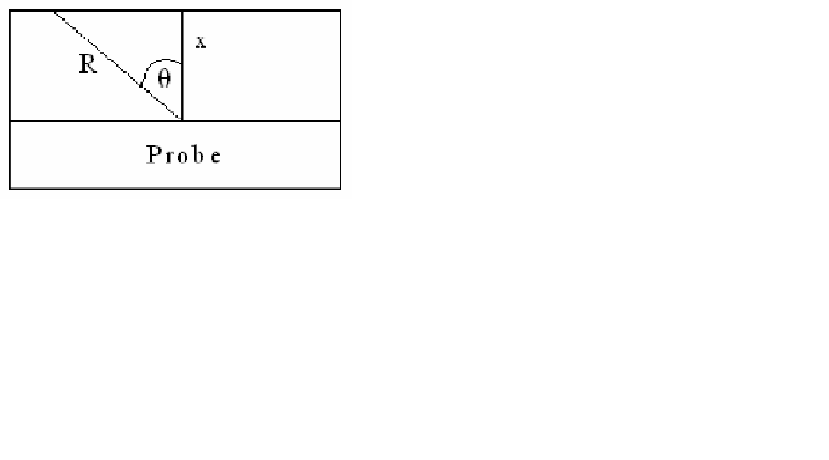
\includegraphics[width=.3\textwidth]{figures/alpha-Korrektur.png}
	\captionof{figure}{For a maximum range R of $\alpha$-particles in the sample there exists a maximum angle $\theta_{max}$ at which particles can still leave the sample.}
\end{minipage}
\vskip0.5cm
Given that $\theta_{max}=arccos\left( \frac{x}{R}\right)$   is the maximum angle allowing $\alpha$-particles to leave the sample, we obtain for the 
solid angle $\Omega$ in which radiation is emitted:
\[\Omega(x)=\int_{0}^{2\pi}d\phi\int_{0}^{\theta_{max}(x)}\sin\theta d\theta = 2\pi\left( 1-\frac{x}{R}\right)\]

For the decay rate n we then obtain:
\[n= \frac{A}{d}\int_{0}^{R}\frac{\Omega(x)}{4\pi}dx = \frac{A_v F}{4\pi}\int_{0}^{R}\Omega(x)dx = \frac{A_v F R}{4}\]
with the thickness $d=\frac{V}{F}$, the surface area $F$, the volume $V$, the activity $A$ and the activity per volume $A_V=\frac{A}{V}$. So we get for the activity:
$$A=\frac{4nV}{FR}$$

With formula (\ref{activity}) we get for the samarium sample:
\begin{align}
	T_{\frac12,\text{Sm}}&=\ln2\cdot\frac{N_{\text{Sm}}RF}{4nV}=\ln2\cdot\frac{2N_{\text{Sm$_2$O$_3$}}h_{\text{rel}}RF}{4nV}=\ln2\cdot\frac{mN_{\text{A}}h_{\text{rel}}RF}{m_{\text{mol}}2nV}
	=\ln2\cdot\frac{N_{\text{A}}h_{\text{rel}}R\rho F}{m_{\text{mol}}2n}\\&
	 =\ln2\cdot\frac{N_{\text{A}}h_{\text{rel}}R\rho\pi d^2}{m_{\text{mol}}8n}\label{halflifeSm}
\end{align}
with the Avogadro constant $N_A$, the natural abundance $h_{rel}$ of $^{147}$Sm and the diameter $d$ of the sample.

\subsubsection{Correction for $\beta$-radiation}\label{betacorrection}

In order to consider the self-absorption effect of $\beta$-radiation the decay rate of the sample is recorded as function of mass, so to say the specific activity  $A_s=A/m$ (Unit Bq/mol)
The decay rate n, that origins from a volume element $F\cdot dx$ in a distance x is dependent on the surface area F, the specific activity $A_s$, the density $\rho$ and the absorption coefficient  $\mu$:  
\[dn\sim A_s\cdot F\cdot \rho\cdot e^{-\mu x}dx\]

Neglecting the energy-dependency of $\mu$ and integrating over height  h=$\frac{m}{\rho F}$ leads to:

\[n(m)\sim\int_{0}^{\frac{m}{\rho F}}A_s F\rho e^{-\mu x}dx = \frac{A_s F\rho}{\mu}\left( 1-exp\left[ -\frac{\mu}{F\rho}m\right] \right)\]

We hence obtain:
\[n(m)= a\left( 1-e^{-bm}\right)\]

In order to take the back-scattering in the aluminium dish into account, we consider the derivative of the function namely the slope of the tangent at the point m=0. The following must hold: 

\[\left. \frac{dn}{dm}\right| _{m=0}=A_s f_B \frac{\Omega}{4\pi}\]
where $\omega$ is the solid angle (in this experiment $2\pi$ )  and $f_B$=1.29 the back-scattering factor of Aluminium.\\

This leads to:
\[\left. \frac{dn}{dm}\right| _{m=0} = ab = \frac{A_s f_B}{2}\]

solving for a and plugging that in we obtain:

\[n(m) = f_B\frac{\Omega}{4\pi}A_s\frac{F\rho}{\mu}\left( 1-exp\left[ -\frac{\mu}{F\rho}m\right] \right) \]

So we get for the activity: $$A=A_s\cdot m=\frac{2abm}{f_B}$$

With formula (\ref{activity}) we get for the half-time of the $\beta^-$-decay of $^{40}$K:
\begin{align*}
	T_{\frac12,\beta^-}&=\frac{\ln2N}{A}=\frac{\ln2Nf_B}{2abm}\\&=\frac{\ln2\frac{m}{m_{mol}}N_Ah_{rel}f_B}{2abm}\\&=\frac{\ln2N_Ah_{rel}f_B}{2abm_{mol}}
\end{align*}

However, the counter tube only detects the $\beta^-$-decay of a sample. The sample used in this experiment also decays via electron capture with a ratio of EC/$\beta^-$=0.12
As the total exponential decay rate is given by:

\[\lambda_{ges} = \lambda_{\beta-} + \lambda_{EC} = \lambda_{\beta-}+0.12\lambda_{\beta-} = 1.12\lambda_{\beta-}\]
the actual half-life will be given by:
\begin{align}
	T_{1/2} &= \frac{T_{1/2,\beta^-}}{1.12}\\
	&=\frac{\ln2N_Ah_{rel}f_B}{2\cdot1.12abm_{mol}}\label{halftimeKa}
\end{align}

 

 

 

 
\newpage
\section{Experimental Set-Up and Procedure }
The pulses detected by the counter tube are proportional to the primary ionisation. They are then converted into voltage signals by a preamplifier (Amplifier 142PC, Firma Ortec) that are again proportional to the primary ionisation. This signal is then converted into a square wave signal with an Amplifier (Amplifier 571, Ortec) using differentiation and integration with a specific time constant (shaping time) $\mu$. This signal is then transferred to a single channel analyzer (TSCA 551, Ortec) with a setting for lower and upper level that determines in which energy range an event is registered. The counter (BNC 2120, National Instrument) is connected with  the program LabView on the computer which allows to vary all essential settings i.e. Voltage, counting time and intervalls.
\vskip 20 pt
\gra[0.8]{Versuchsaufbau}{Experimental Set-Up}
\subsection{Used samples}

\subsubsection{Characteristic of the Counter tube}\label{uranium}
To record the characteristic of the Counter Tube ${}^{238}$Uranium is used. It makes up 99.275\% of the natural Uranium.
With a half-life of $T_{1/2}({}^{238}U)=4.468\cdot 10^9$a it transforms via  $\alpha$-decay to ${}^{234}$Thorium. The energy of the $\alpha$-particle is about 4MeV in this process. According to \ref{alpha} this process is described as:

\[{}^{238}_{92}U \rightarrow {}^{234}_{90}Th + {}^4_2He\]

Thorium then decays via $\beta$-decay  to ${}^{234}$Palladium with a half-time of  $T_{1/2}({}^{234}Th)$=24,1d, which again decays via  $\beta$-Zerfall into ${}^{234}$Uranium. According to \ref{beta} this processes are written as follows:

\[{}^{234}_{90}Th \rightarrow {}^{234}_{91}Pd + e^- + \bar{\nu_e}\]

\[{}^{234}_{91}Pd \rightarrow {}^{234}_{92}U + e^- + \bar{\nu_e}\]

The energy of these decays is given by 80keV-200keV for the Thorium decay and up to 1250keV for Palladium accordingly.


\subsubsection{$\alpha$-radiator}

In this experiment ${}^{147}$Samarium that makes up 15\% of the natural Samarium is used as $\alpha$-radiator. The used sample consists of $Sm_2O_3$ and has a purity of 99\%. Samarium has a half-life of  $T_{1/2}({}^{147}Sm)=1.06\cdot10^{11}$a. It decays into ${}^{143}$Neodym (stable) transmitting an $\alpha$-particle with an energy of about 2MeV.

\[{}^{147}_{62} \rightarrow {}^{143}_{60}Nd + {}^4_2He\]

\subsubsection{$\beta$-radiator}\label{kaliumdurchfuehrung}
As $\beta$-radiator we use ${}^{40}$Kalium with a relative  mass portion of 0.0118\%. The sample used in the Experiment is KCl. 
${}^{40}$Kalium can decay via two decays: Either via $\beta^-$-Zerfall to ${}^{40}$Calcium or via electron capture to ${}^{40}$Argon:

\[{}^{40}_{19}K \rightarrow {}^{40}_{20}Ca + e^- + \bar{\nu_e}\]
\[{}^{40}_{19}K + e^- \rightarrow {}^{40}_{18}Ar + \bar{\nu_e}\]

The ratio for the two decays is $\frac{EC}{\beta-}=0.12$.\\

As discussed in chapter \ref{betacorrection} the measured counting rate of Kalium is mass-dependent. That's why we measure the counting rate of Kalium for different masses and calculate the half-life out of an exponential fit.


\newpage
\section{Analysis}

\subsection{Counter Tube Characteristics}

\subsubsection{Uranium}
As discussed in chapter \ref{uranium} we use $^{238}$Uranium to get the characteristics of the counter tube.
\gra{zaehlrohr-uran}{Counter tube characteristics of $^{238}$U\label{curan}}
In figure \ref{curan} we see two plateaus. The first plateau comes from the $\alpha$-decay of $^{238}$U and the second plateau shows the $\beta$-decay of $^{234}$Th and $^{234}$Pd. 

\subsubsection{Background}\label{untergrund}
We measured the background radiation by putting an empty aluminium dish inside the counter tube.
\gra{zaehlrohr-untergrund}{Counter tube characteristics of the background radiation\label{background}}
In figure \ref{background} we see that the background is very small. The background counting rates are about 3 orders of magnitude smaller than the counting rates of the uranium sample. So we would not be able to see any change in the position of the plateaus if we substracted the background from the counter tube characteristics of the uranium sample.\\

Additionally the time for measuring the background is very short, so we don't get significant background counting rates. We see in figure \ref{background} that the counting rates scatter a lot and won't better our values.
\newpage
\subsubsection{Samarium}
Now we tried to get the working point for the Samarium measurements. Therefor we measured the counter tube characteristics of Samarium in a span starting at the beginning of the $\alpha$-plateau of uranium and ending on the beginning of the $\beta$-plateau of uranium.

\gra{zaehlrohr-samarium}{Counter tube characteristics of $^{147}$Sm \textcolor{blue}{(corrected with the background)}\label{csamarium}}

In figure \ref{csamarium} we plotted the counter tube characteristics of $^{147}$Sm once original and once corrected by the background seen in figure \ref{background}. Since the corrected data scatters a lot and has very big error bars (as discussed in chapter \ref{untergrund}) we can't really use the corrected data to set our working point. So we assumed an almost linear behavior in the range of $U=2300\,\mathrm{V}$ and $U=2900\,\mathrm{V}$. Considering the $\alpha$-plateau from figure \ref{curan} we set the working point for Samarium to $U=2500\,\mathrm{V}$
\newpage
\subsubsection{Kalium}
We also measured the counter tube characteristics of Kalium to determine the working point for the Kalium measurements. We started at the beginning of the $\beta$-plateau and stopped at $U=4000\,\mathrm{V}$.
\gra{zaehlrohr-kalium}{Counter tube characteristics of $^{40}$K \textcolor{blue}{(corrected with the background)}\label{ckalium}}

In figure \ref{ckalium} we see that the counting rate seems to be constant between $U=3300\,\mathrm{V}$ and $U=4000\,\mathrm{V}$ with one outlier at $U=3800\,\mathrm{V}$. The correction does not essentially change this behavior, so we choose our working point at $U=3500\,\mathrm{V}$.
\newpage
\subsection{Half-life of Samarium}
With formula (\ref{halflifeSm}) we can now calculate the half-life of Samarium out of the measured counting rate. We use the following constants
\begin{align*}
	N_{\text{A}}&=6.022\cdot10^{23}\\
	h_{\text{rel}}&=0.1487\,^{\cite{anleitung}}\\
	R\rho&=0.04025&\text{(calculated out of the known values for air)}\\
	m_{\text{mol}}&=0.34872
\end{align*}
and the following measurement data:
\begin{align*}
	d&=(2.877\pm0.002)\cdot10^{-2}\mathrm{m}\\
	n&=(0.416\pm0.009)\,\mathrm{s^{-1}}
\end{align*}
We get the following result: 
\begin{align*}
	T_{\frac12,\text{Sm}}&=\ln2\cdot\frac{N_{\text{A}}h_{\text{rel}}R\rho\pi d^2}{m_{\text{mol}}8n}\\&=1.93\cdot 10^{11}\text{ years}
\end{align*}
The error on $T_{\frac12,\text{Sm}}$ we get with the gaussian error propagation on the Poisson errors of the counting rate: 
\begin{align*}
	s_{T_{\frac12,\text{Sm}}}&=T_{\frac12,\text{Sm}}\cdot\sqrt{\left(2\frac{s_d}{d}\right)^2+\left(\frac{s_n}{n}\right)^2}\\&=0.04\cdot 10^{11}\text{ years}
\end{align*}

So our result for the half-life of Samarium is:
\begin{align*}
	T_{\frac12,\text{Sm}}&=\left(1.93\pm0.04\right)\cdot10^{11}\text{ years}
\end{align*}
\newpage
\subsection{Half-life of Kalium}
As described in chapter \ref{kaliumdurchfuehrung} we measured the counting rate of Kalium for different masses. The counting rate relates to the mass as following: 
\begin{align}
	n=a(1-e^{-bm})\label{fitfunction}
\end{align}

\gra{kalium}{Counting rate in dependence of the mass with an exponential fit\label{kalium}}

Fitting formula (\ref{fitfunction}) to the data (see figure \ref{kalium}) gives us the following parameters:
\begin{align*}
	a&=4.4\,\mathrm{s^{-1}}\\
	b&=2119\,\mathrm{kg^{-1}}
\end{align*}
with the following covariance matrix
\begin{align*}
\sigma&=\left(
	\begin{matrix}
		0.25&-705\\
		-705&2250000
	\end{matrix}
\right)
\end{align*}

We have the following constants:
\begin{align*}
	N_{\text{A}}&=6.022\cdot10^{23}\\
	h_{\text{rel}}&=0.000118\,^{\cite{anleitung}}\\
	f_B&=1.29\\
	m_{\text{mol}}&=0.07455
\end{align*}

So we can calculate the half-life with formula (\ref{halftimeKa}):
\begin{align*}
	T_{\frac12,\text{Ka}}&=\frac{\ln2N_Ah_{rel}f_B}{2\cdot1.12abm_{mol}}\\
	&=1.3\cdot10^{9}\,\text{years}
\end{align*}
The error on $T_{\frac12,\text{Ka}}$ we get once again with the gaussian error propagation: 
\begin{align*}
	s_{T_{\frac12,\text{Ka}}}&=\sqrt{\sum_{i,j=\{a,b\}}\left(\del[T_{\frac12,\text{Ka}}]{i}\right)\left(\del[T_{\frac12,\text{Ka}}]{j}\right)\sigma_{ij}}\\
	&=0.8\cdot10^9\,\text{years}
\end{align*}
So our result for the half-life of Samarium is:
\begin{align*}
T_{\frac12,\text{Ka}}&=\left(1.3\pm0.8\right)\cdot10^{9}\text{ years}
\end{align*}
\newpage
\section{Summary/Discussion}
Our results for the half-lifes are
\begin{align*}
	T_{\frac12,\text{Sm}}&=\left(1.93\pm0.04\right)\cdot10^{11}\,\text{years}\\
	T_{\frac12,\text{Ka}}&=\left(1.3 \pm0.8 \right)\cdot10^{9} \,\text{years}
\end{align*}
The literature value according to \cite{anleitung} are
\begin{align*}
	T_{\frac12,\text{Sm},\text{lit}}&=1.06\cdot10^{11}\,\text{years}\\
	T_{\frac12,\text{Ka},\text{lit}}&=1.28\cdot10^{9} \,\text{years}
\end{align*}

One can see that our result for the half-life of Samarium is in the same order of magnitude but about a factor 1.5 bigger than the literature value. So we have a systematic error that we have not considered during the experiment. Since we do not know the exact structure from the counter tube, maybe the sample was not exactly in the opening so that the actual area is smaller than the measured one.\\
Also we do not know how pure the Sm$_2$O$_3$ really is. There could be a contamination caused by the putting back of the samples.\\

The result for the half-life of Kalium however is very good compared to the literature value, although it has a very large error. The big error is caused by the high scattering of our counting rates (see figure \ref{kalium}), which we cannot explain. The scattering is higher than our statistical errors given by the Poisson errors would let us assume.\\

So probably there also is an unknown error which has an statistical effect on our measurements. Since the position of the sample inside the apparatus isn't always the same it's also possible that we did not always have the whole sample under the opening and lost an unknown mass for our measurements.

\newpage
\section{Attachments}









\subsection{Sourcecode}

\ 

%\subsubsection{$\alpha$-Plateau Samarium}
%\lstinputlisting{data/Americium_1.TKA}


%\newpage
%\subsection{Quellcode (MATLAB)}
%\lstinputlisting[language=MATLAB]{Rohdaten/alpha.m}


%\begin{minipage}{\textwidth}
%\centering
%\includegraphics[width=0.9\textwidth]{figures/IMG_20151002_141014.jpg}
%\end{minipage}

\subsection{Measurement protocol}\label{laborbuch}
\begin{minipage}{\textwidth}
	\centering
	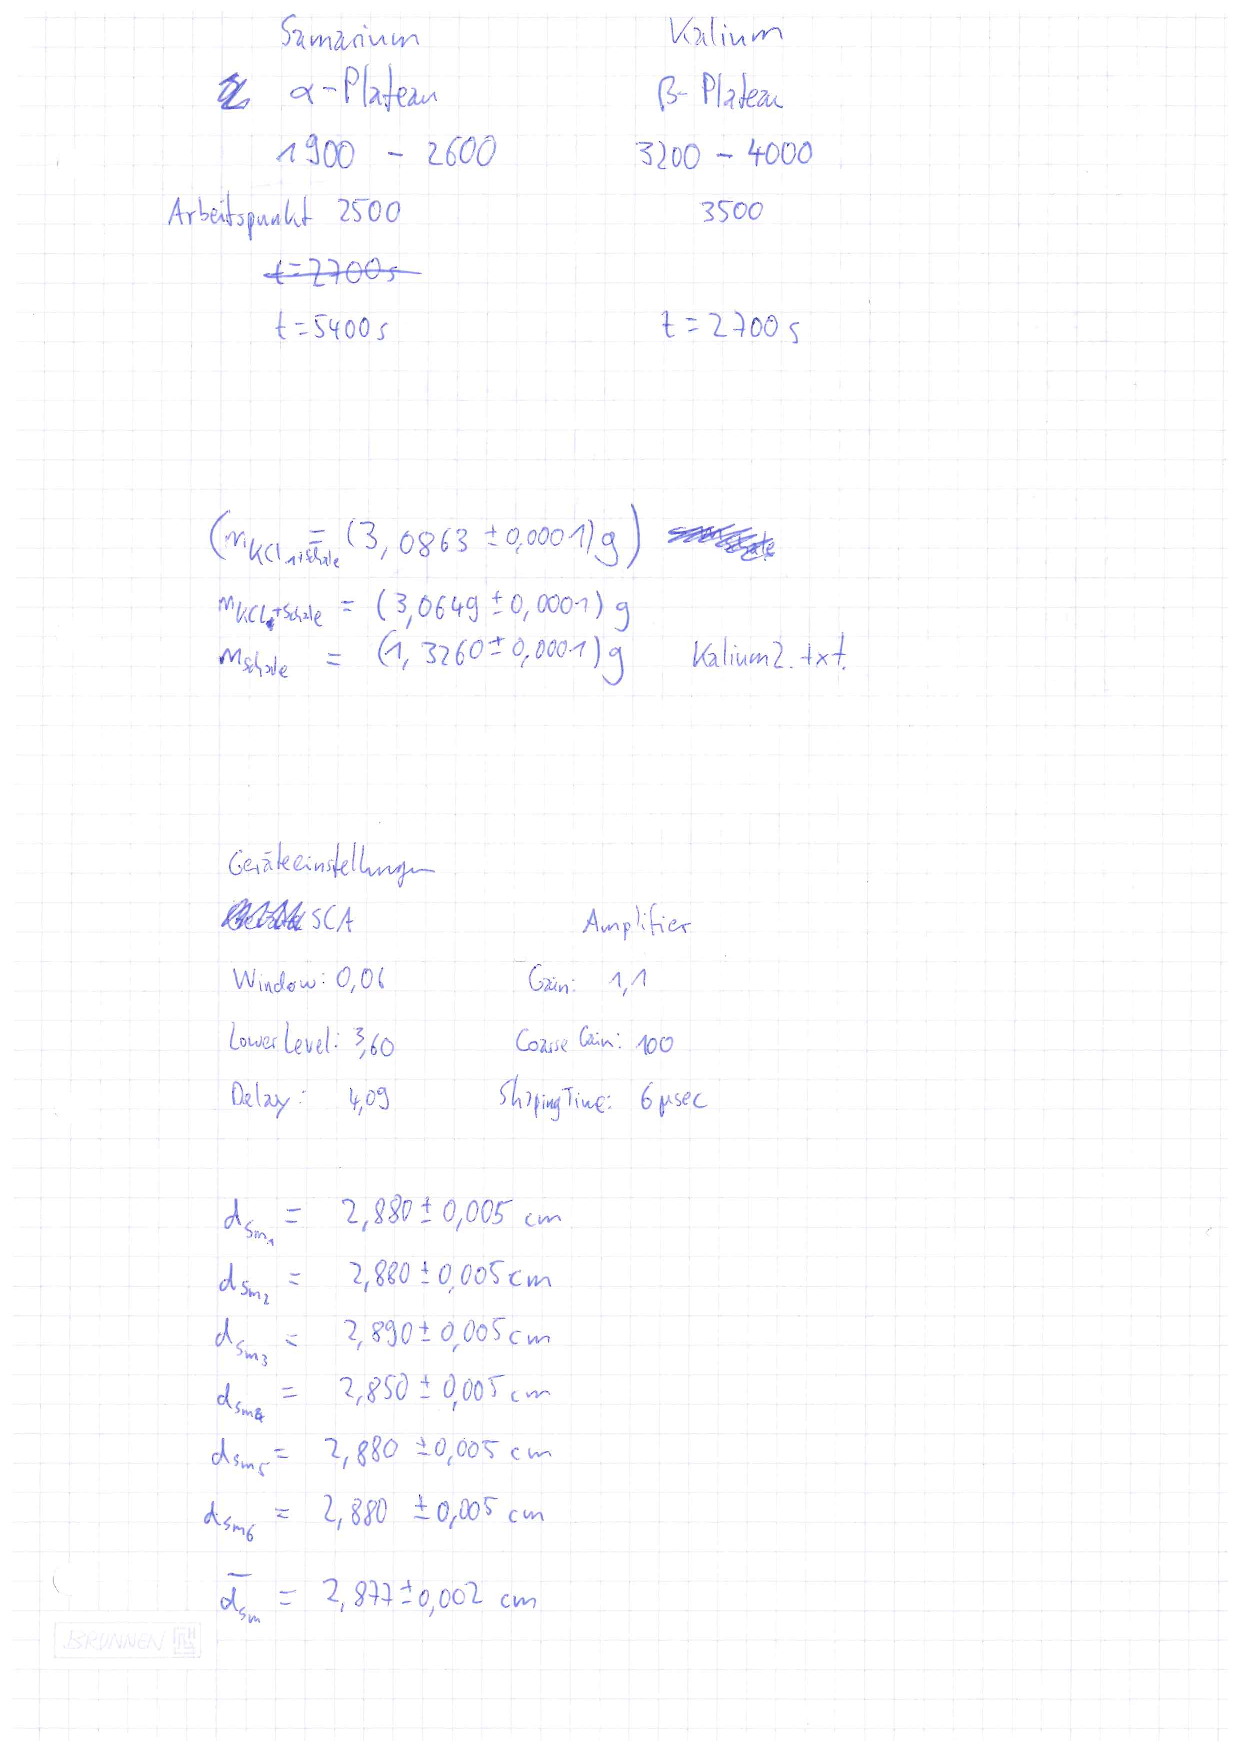
\includegraphics[width=0.9\textwidth]{figures/Laborbuch-1.pdf}
\end{minipage}
\begin{minipage}{\textwidth}
	\centering
	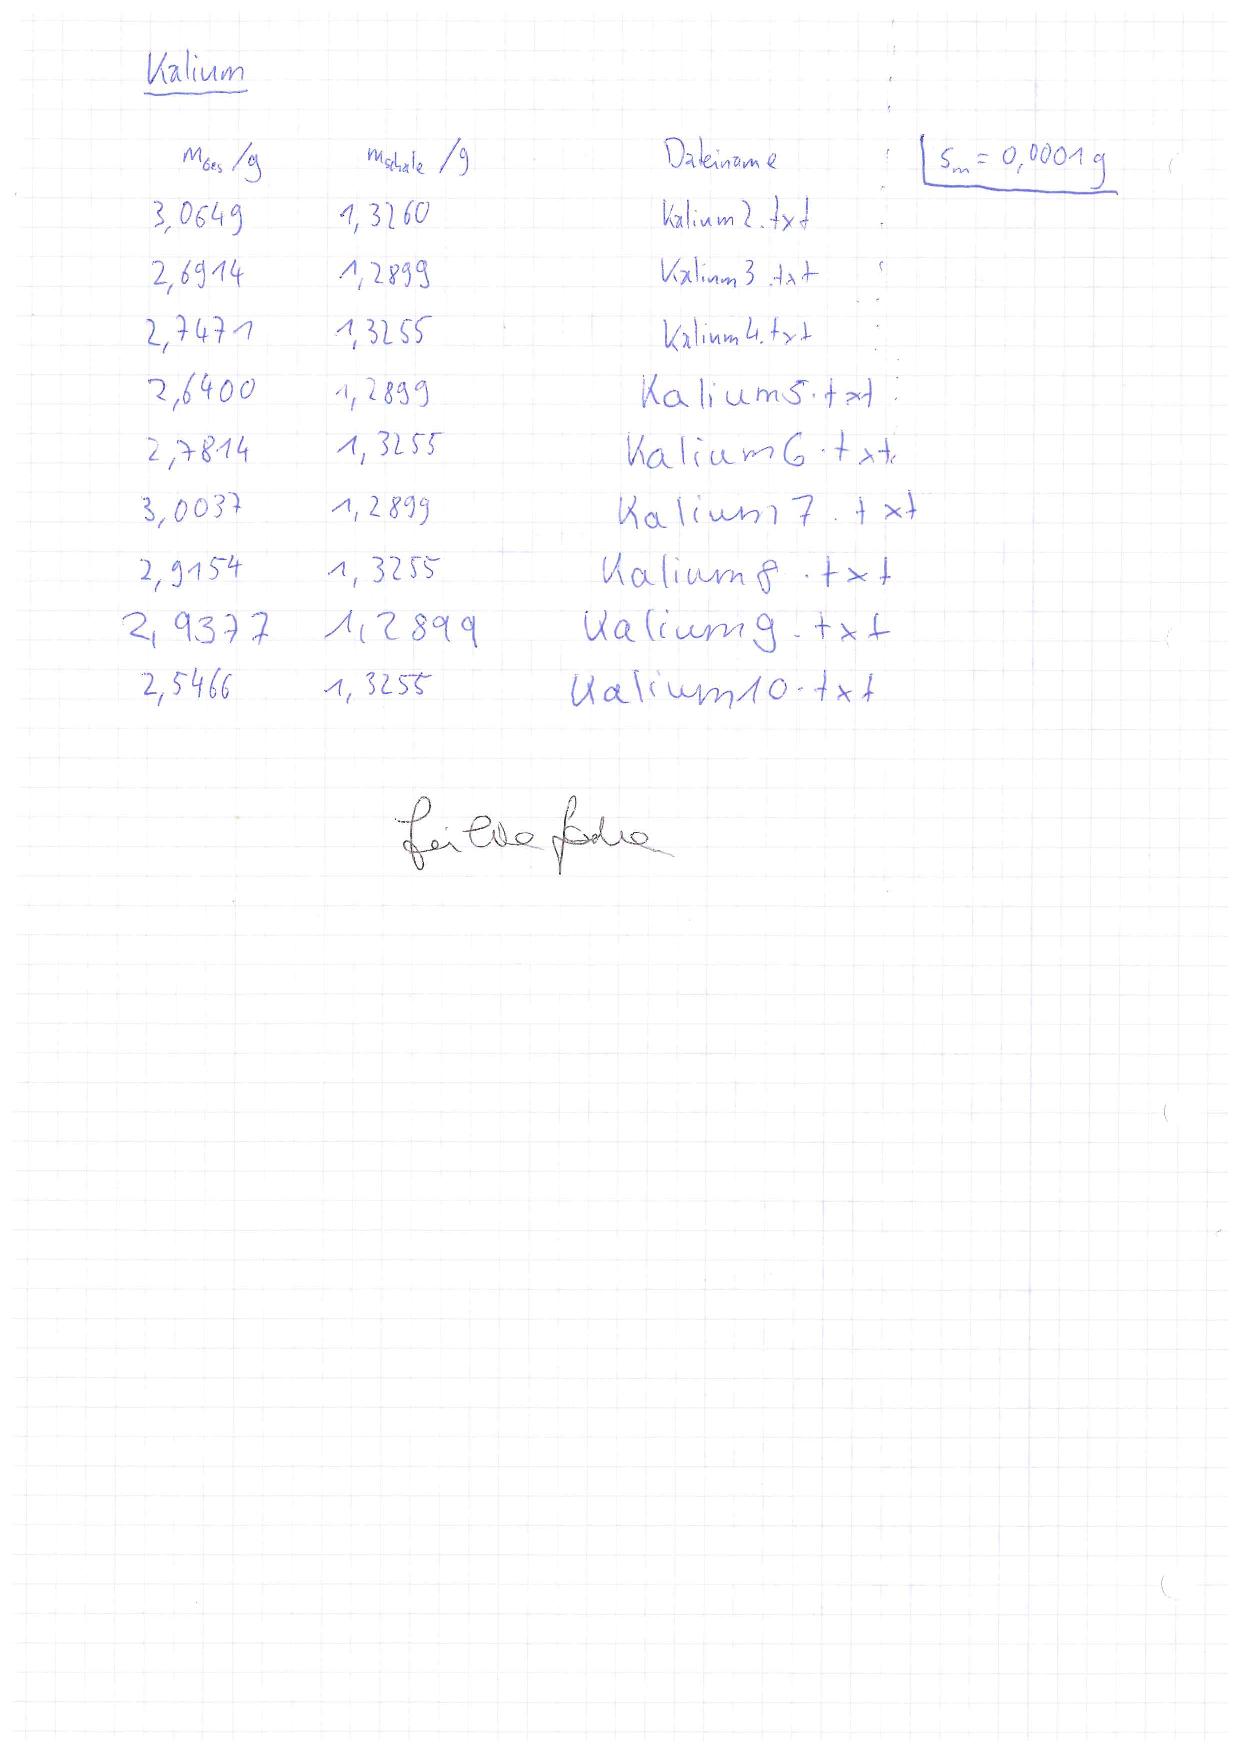
\includegraphics[width=0.9\textwidth]{figures/Laborbuch-2.pdf}
\end{minipage}
\newpage
\listoffigures

%Literatur----------------------------------------------------------------------------------------------------------

%\cite{les}
\newpage
\thispagestyle{empty}
\begin{thebibliography}{9}

\bibitem{anleitung}
\emph{Versuchsanleitung Fortgeschrittenen Praktikum: Lange Halbwertszeiten},
Albert-Ludwigs-Universität Freiburg,
2012

\bibitem{staat}
Tobijas Kotyk,
\emph{Versuche zur Radioaktivität im Physikalischen Fortgeschrittenen Praktikum an der Albert-Ludwigs-Universität Freiburg},
Albert-Ludwigs-Universität Freiburg,
1979
  
%\bibitem{molmasse}
%  \emph{http://www.convertunits.com/molarmass/<ELEMENTNAME AUF ENGLISCH>}, Stand 28.09.2015
  

\end{thebibliography}

\end{document}